\documentclass[14pt, aspectratio=169]{beamer}

\usepackage[T2A]{fontenc}
\usepackage[utf8]{inputenc}
\usepackage[bulgarian]{babel}
\usepackage[nointegrals]{wasysym}

\usetheme{tues}

\graphicspath{{assets/}}

\definecolor{bibnote}{HTML}{627293}

\usepackage{tikz}

\title{Въведение в операционните системи}
\subtitle{Операционни системи}
\author{Ангел Пенчев}
\institute{ТУЕС, XI\textsuperscript{А}}
\date{\today}

\begin{document}

\begin{frame}
  \tableofcontents
\end{frame}

\section{Какво е операционна система?}

\begin{frame}{Видове софтуер}
  \emph{Какво е системно програмиране?}
  \bigskip

  \onslide<2>{%
    \renewcommand{\arraystretch}{1.25}%
    \small
    \noindent
    \begin{tabularx}{\textwidth}{@{}XXX@{}}
      \toprule
      \textbf{Компонент} & \textbf{Интерфейс} & \textbf{Функции} \\
      \midrule
      Приложна програма & Към потребителя - конзола, графично & Бизнес логика \\
      Библиотеки за общо предназначение & Прост
        & Общи - низове, памет, математика и т.н. \\
      Библиотеки за достъп до хардуер & Логическо устройство
        & Управление на конкретен хардуер \\
      \bottomrule
    \end{tabularx}}
\end{frame}

\begin{frame}{Какво е операционна система?}
  \begin{itemize}
    \item Няма една общоприета дефиниция. По-лесно е да я опишем чрез това,
      което прави:
      \begin{itemize}
        \item управлява хардуера на системата;
        \item дава на програмите \emph{непряк} достъп до него чрез интерфейс
          (API) - и чрез същия интерфейс ги ограничава.
      \end{itemize}
  \end{itemize}
\end{frame}

\begin{frame}{Ограничения чрез интерфейса}
  \begin{itemize}
    \item \texttt{open()} - ОС проверява правата за достъп до файла и може да
      откаже с грешка. \texttt{read()} и \texttt{write()} после работят само с
      вече отворения файл.
    \item \texttt{malloc()} и \texttt{free()} \textbf{не} са системни
      извиквания, а функции от \texttt{libc}. Когато им трябва още памет, те я
      искат от ядрото с \texttt{brk()} или \texttt{mmap()} - и ядрото решава
      дали да я даде.
    \item Ако програма достъпи памет, която не е нейна, процесорът сигнализира
      на ядрото и то я спира - \texttt{Segmentation fault} (сигнал
      \texttt{SIGSEGV}).
  \end{itemize}
\end{frame}

\begin{frame}{Какво е операционна система?}
  \begin{itemize}
    \item Операционната система (ОС) е софтуер, който споделя и разпределя
      ресурсите на хардуера между различни програми.
    \item Тези програми получават възможност от ОС да не се съобразяват с
      останалите агенти на системата, а само със самата ОС.
    \item Споделянето на ресурсите се осъществява чрез \emph{изолация} и/или
      чрез \emph{заявки}.
    \item \emph{Изолацията} е метод, чрез който ОС показва даден ресурс само и
      единствено на неговия \emph{собственик}.
  \end{itemize}
\end{frame}

\begin{frame}{Какво е операционна система?}
  \begin{itemize}
    \item \emph{Методът на заявките} изисква изрично обръщения на всички
      програми към един и същ ресурс едновременно. Този вид споделяне бива два
      вида - \emph{последователно} (или блокиращо, или синхронно) и
      \emph{паралелно} (или асинхронно). При първото програмата блокира, докато
      не завърши изпратената заявка, докато при второто заявката се поставя в
      опашка за изпълнение и програмата няма контрол в какъв момент точно ще
      бъде изпълнена.
  \end{itemize}
\end{frame}

\begin{frame}{Какво е операционна система?}
  \begin{tabular}{@{}lll@{}}
    \toprule
    \textbf{Ресурс} & \textbf{Абстракция} & \textbf{Метод на споделяне} \\
    \midrule
    Процесор & Нишки & Изолация (и времеделене) \\
    Памет & Адресно пространство & Изолация \\
    Диск & Файлова система & Заявки \\
    Мрежа & Сокети & Заявки \\
    Принтер & Логически принтер & Заявки (асинхронни) \\
    \bottomrule
  \end{tabular}
\end{frame}

\begin{frame}{Какво е операционна система?}
  Изискванията към една ОС още включват -
  \begin{itemize}
    \item Скорост - цената за изпълнение на ОС трябва да бъде минимална.
    \item Надеждност - от издръжливостта на ОС зависят и приложенията.
    \item Изолация между изпълняващите се приложения с цел сигурност.
      Същевременно, начин за споделяне на данни между приложения с цел
      кооперация.
    \item Абстрахиране на конкретния хардуер с цел преносимост.
    \item Удобен интерфейс, за да бъде лесна за употреба.
  \end{itemize}
\end{frame}

\begin{frame}{Многозадачност}
  \begin{itemize}
    \item Очакваме много програми да работят едновременно, но едно процесорно
      ядро изпълнява инструкциите последователно - една програма в даден
      момент.
    \item Илюзията се постига с \emph{времеделене}: таймер предизвиква
      прекъсване на всеки няколко милисекунди, ядрото получава управлението и
      може да даде процесора на друга програма.
    \item Програмите се редуват толкова често, че изглеждат едновременни -
      това е \emph{конкурентност}, не \emph{паралелизъм}.
    \item Многоядрените процесори наистина изпълняват няколко програми
      паралелно - и на всяко ядро отново има времеделене.
  \end{itemize}
\end{frame}

\begin{frame}{Многопотребителност}
  \begin{itemize}
    \item Един компютър често се ползва от няколко потребители - понякога
      едновременно, например сървър, към който се свързват по SSH.
    \item ОС знае кой потребител е стартирал всеки процес и кой притежава
      всеки файл.
    \item Така пази данните и програмите на всеки потребител от останалите -
      това е изолация, но между хора, а не само между програми.
  \end{itemize}
\end{frame}

\begin{frame}[allowframebreaks]{Структура на ОС}
  След като сме описали задачите, които една ОС трябва да решава, нека опитаме
  да си представим как изглежда горе-долу една такава.

  Нека разгледаме един крайно опростен пример. Имаме приложения, които искат
  да пишат по диска, за да запазват потребителски данни. ОС, в която се
  изпълняват, предоставя интерфейс за работа с диска - приложенията извикват
  \texttt{disk\_write(sector, data)} и ОС се грижи за магията.

  Имаме две непосредствени следствия-проблеми. От една страна това означава,
  че приложение А може да реши да използва сектор 42 и приложение Б да си
  хареса същия сектор. Така те ще бъдат в постоянно състояние на
  \emph{състезание} (на англ. race condition) за данните на сектор 42.

  От втора страна, щом това е просто функция, която може да се извика от
  всеки, то системата е много лесна за компрометиране - произволна програма
  може да изтрие данните на потребителя. Със сигурност нежелан ефект!

  Достигаме до много важен извод - ОС \textbf{не} е просто библиотека с
  функции, които се „грижат за хардуера“. \emph{Откъде точно произлиза
    разликата обаче?}

  \framebreak

  Разликата е, че не всяка програма трябва да може да пише по диска каквото и
  където си пожелае. Това трябва да бъде допустимо при силни ограничения - все
  пак не бива да го забраняваме; дискът наистина е за писане. \emph{Как
    решаваме този проблем?}

  \bigskip
  Понеже разбираме, че трябва дискът да бъде споделен между множество
  програми, си спомняме, че това се случва чрез \emph{заявки} към
  \emph{абстракцията} на диска, а именно - \emph{файловата система}. Така
  решаваме единия проблем.
\end{frame}

\begin{frame}{Структура на ОС}
  Вторият проблем, който представихме, се отнася до сигурността на ОС.
  Решаваме го по следния начин. Въвеждаме понятието \underline{ниво на
    привилегия} (на англ. privilege level или още protection rings). Това е
  свойство на изпълняваща се програма - казваме, че се изпълнява с някакво
  ниво на привилегия.
\end{frame}

\begin{frame}{Структура на ОС}
  \begin{columns}[T]
    \begin{column}{0.48\textwidth}
      \begin{figure}
        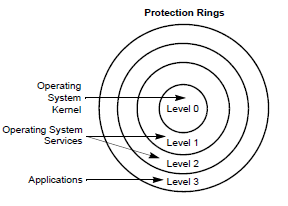
\includegraphics[height=0.42\textheight]{x86-protection-rings}
        \caption{x86 Нива на привилегия}
      \end{figure}
    \end{column}
    \begin{column}{0.48\textwidth}
      \begin{figure}
        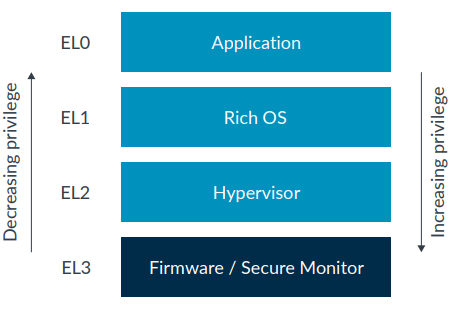
\includegraphics[height=0.42\textheight]{arm-exception-levels}
        \caption{ARM Нива за изключения}
      \end{figure}
    \end{column}
  \end{columns}
  \small
  x86 има 4 нива, но Linux и Windows използват само две: ниво 0 за ядрото и
  ниво 3 за приложенията.
\end{frame}

\begin{frame}[allowframebreaks]{Структура на ОС}
  И тогава решението на проблема ни е много просто - за да изпълнява
  \texttt{disk\_write()} (от предходния ни пример), изискваме програмата да се
  изпълнява с ниво на привилегия, което позволява това.

  Както уточнихме вече обаче приложенията не се изпълняват с ниво на
  привилегия, което позволява това. И това е по дизайн.

  Нуждаем се от метод за „промяна на нивото на привилегия“ - изпълняваме си
  приложението, вършейки позволени операции (математически операции, работа с
  низове, взаимодействие с потребител), и в някакъв момент искаме да извикаме
  „забранената“ функция \texttt{disk\_write()}. След като функцията приключи
  работата си, искаме нивото на привилегия да се смени отново - този път към
  началното си състояние.

  Този механизъм се нарича \underline{системно извикване} (на англ. system
  call или накратко syscall). Чрез него потребителско приложение инициира
  работа за ОС. Казваме, че приложението се изпълнява в
  \underline{потребителски режим} (на англ. user mode), а ОС - в
  \underline{режим на ядрото} (на англ. kernel mode). Онази част от ОС, която
  се изпълнява в режим на ядрото, наричаме \underline{ядро} (на англ.
  kernel). При изпълнение в режим на ядрото програмата има достъп до цялата
  системна памет и всички инструкции на процесора, докато при потребителския
  режим ОС се налагат ограничения.

  Нека имаме едно примерно системно извикване \texttt{S()}. Технологията на
  извикване на \texttt{S()} е следната. Когато потребителско приложение А
  желае да изпълни \texttt{S()}, то трябва да задейства \underline{софтуерно
    прекъсване „капан“} (на англ. trap software interrupt), при което
  процесорът ще съхрани състоянието на А, ще премине към режим на ядрото и ще
  премине към изпълнение на обработка на софтуерното прекъсване. При
  обработката на софтуерното прекъсване ще се изпълни работата на
  \texttt{S()}, след което процесорът ще изпълни специална инструкция за
  излизане от капана, ще възвърне състоянието на приложението и то ще
  продължи работата си.

  Забелязваме обаче един важен детайл. При извикването на \texttt{S()} не
  можем просто да посочим неговия адрес. \emph{Защо?}

  Например, ако желаем да отворим файл, за който нямаме права, можем да
  посочим адрес, съответстващ на функцията след проверката за
  правоспособност. Така получаваме способност за отваряне на произволен файл,
  заобикаляйки всякакви проверки за сигурност. Това се нарича
  \underline{уязвимост} (на англ. vulnerability).

  Решението на този проблем е просто. Ядрото използва фиксирана таблица за
  своите системни извиквания. Потребителско приложение уточнява единствено
  индекса на системното извикване, което иска да се изпълни, а ядрото намира
  адреса на съответстващата функция при обработката на софтуерното
  прекъсване.

  Така изяснихме общата постановка на комуникация между ОС и приложенията,
  които ОС управлява.

  Примери за системни извиквания в Linux са \texttt{write}, \texttt{mmap},
  \texttt{shmat} и \texttt{dup}. На x86-64 са
  \weblink{https://filippo.io/linux-syscall-table/}{около 400}. Може да се
  запознаете по-обстойно с всеки от тях, използвайки командата \texttt{man 2
    <syscall>}. Можете да разгледате системните извиквания, които Linux
  ядрото предоставя, търсейки макрото \texttt{SYSCALL\_DEFINE}\emph{x}, където
  \emph{x} е цяло число от 0 до 6 (броя параметри) в хранилището на кода -
  \weblink{https://github.com/torvalds/linux.git}{torvalds/linux.git} или в
  индексиращата система
  \weblink{https://elixir.bootlin.com/linux/v6.16/source}{Bootlin}. Да
  отбележим, че когато извикаме например \texttt{write} в своя програма това
  \textbf{не} е системното извикване, както очакваме. Всъщност това е
  функция, дефинирана в стандартната библиотека \texttt{glibc}, която
  извършва описания от нас процес с поставянето на число на определено място
  и предизвикване на софтуерно прекъсване. Такива функции се наричат
  \underline{обвивка} (на англ. wrapper или jacket).

  В macOS ситуацията е подобна на тази в Linux, поради споделения им
  произход. Можете да разгледате системните извиквания в хранилището на кода
  -
  \weblink{https://github.com/opensource-apple/xnu/blob/master/bsd/kern/syscalls.master}{apple/xnu.git}.
  Там вместо подход с макроси, използват генератор на код.

  В Windows обичайно се използват различни имена на понятията, но
  фундаментално идеята е същата. Наместо системно извикване, популярният
  термин е системна услуга (на англ. system service). Технологията на
  извикване е сходна - числото, подадено от извикващия се използва от
  \emph{диспечера на системни услуги}, за да индексира таблица със самите
  функции, имплементиращи системното извикване. Самите системни извиквания
  са недокументирани официално, но до известна степен следват т.нар. Native
  API, имплементиран в \texttt{NTDLL.dll}, което е „най-ниската точка“,
  изпълняваща се в потребителски режим. Примери за системни услуги в Windows
  са \texttt{NtReadFile} и \texttt{NtWaitForSingleObject}.
\end{frame}

\begin{frame}{Ядрото}
  \begin{itemize}
    \item Ядрото е единствената част от ОС, която работи в режим на ядрото -
      всичко останало работи в потребителски режим.
    \item То управлява хардуера пряко, включително чрез драйверите на
      устройствата.
    \item В Linux и Windows драйверите работят в режим на ядрото - в Linux
      често като модули, зареждани при нужда. Грешка в драйвер може да срине
      цялата система.
    \item В микроядрата (MINIX 3, QNX) драйверите са отделни програми в
      потребителски режим - по-бавно, но по-надеждно.
  \end{itemize}
\end{frame}

\begin{frame}{Системни извиквания - примери}
  \begin{center}
    \small
    \begin{tabular}{@{}ll@{}}
      \toprule
      \textbf{Група} & \textbf{Системни извиквания} \\
      \midrule
      \seg Процеси & \texttt{fork}, \texttt{execve}, \texttt{waitpid},
        \texttt{exit} \\
      \seg Файлове & \texttt{open}, \texttt{close}, \texttt{read},
        \texttt{write}, \texttt{lseek} \\
      \seg Файлова система & \texttt{stat}, \texttt{mkdir}, \texttt{rmdir},
        \texttt{link}, \texttt{unlink}, \texttt{mount}, \texttt{chmod} \\
      \bottomrule
    \end{tabular}
  \end{center}
  \begin{itemize}
    \item В C ги извикваме чрез обвивките от \texttt{libc} със същите имена.
      Понякога обвивката вика друго извикване - например \texttt{waitpid()} в
      Linux на x86-64 използва \texttt{wait4}.
    \item Функциите \texttt{execl()}, \texttt{execvp()} и т.н. са обвивки
      около едно и също извикване - \texttt{execve}.
  \end{itemize}
\end{frame}

\begin{frame}{Обвивка (shell)}
  \begin{itemize}
    \item Обвивката е програмата, чрез която потребителят работи с ОС - приема
      команди и ги изпълнява чрез системни извиквания към ядрото.
    \item Може да е текстова (\texttt{bash}, \texttt{zsh}, PowerShell) или
      графична (GNOME Shell, Windows Explorer).
    \item Освен нея ОС включва системни библиотеки (\texttt{libc}), помощни
      програми (\texttt{ls}, \texttt{cp}, \dots) и фонови услуги.
    \item В GNU/Linux Linux е ядрото, а GNU дава почти всичко останало -
      \texttt{libc}, основните команди, \texttt{bash}, компилатора.
  \end{itemize}
\end{frame}

\subsection{Упражнение 1}

\begin{frame}{Упражнение}
  \emph{Забележка:} Понеже все още не сме преминали през темите относно
  \texttt{C}, задачките ще изискват само най-елементарни познания и вярвам, че
  ще се справите \smiley.
  \begin{itemize}
    \item Напишете програма, която приема от стандартния си вход три аргумента
      - име на файл, отместване във файла и низ. Използвайки обвивките на
      системните извиквания за работа с файл - {\rmfamily\textsc{отваряне}},
      {\rmfamily\textsc{писане}} и {\rmfamily\textsc{затваряне}}, програмата
      записва на посоченото отместване данните във файла и приключва.
      \answer{Под Linux и Mac OS използвайте open, write и close, а под
        Windows - CreateFileA, WriteFile и CloseHandle.}
  \end{itemize}
\end{frame}

\begin{frame}{Упражнение}
  \begin{itemize}
    \item Използвайте програма за проследяване на системните извиквания, за да
      разгледате хода на програмата си. В Windows използвайте
      \texttt{Procmon}, в Mac OS - \texttt{sudo dtruss}, а в Linux
      \texttt{strace}. Ако имате други предпочитания, нямам против.
    \item \emph{Забележка (Windows):} Това, което се вижда в колоната
      „Operation“ в \texttt{Procmon} не са системните услуги. Същевременно при
      \emph{\textless десен клик\textgreater} $\rightarrow$ \emph{Stacks} се виждат ясно всички
      извиквания, които се пораждат от функцията, както и това в какъв момент
      точно се преминава към режим на ядрото.
  \end{itemize}
\end{frame}

\begin{frame}
  \begin{figure}
    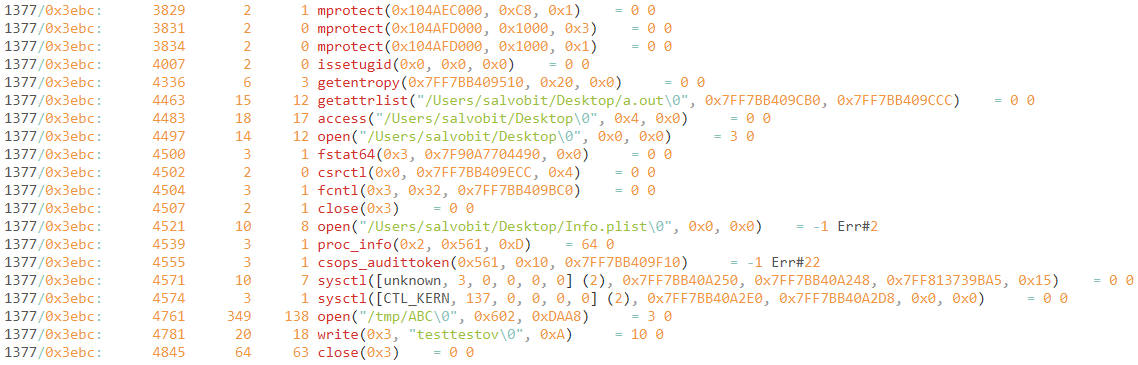
\includegraphics[width=\textwidth]{dtruss}
    \caption{Dtruss (откъс)}
  \end{figure}
\end{frame}

\begin{frame}
  \begin{figure}
    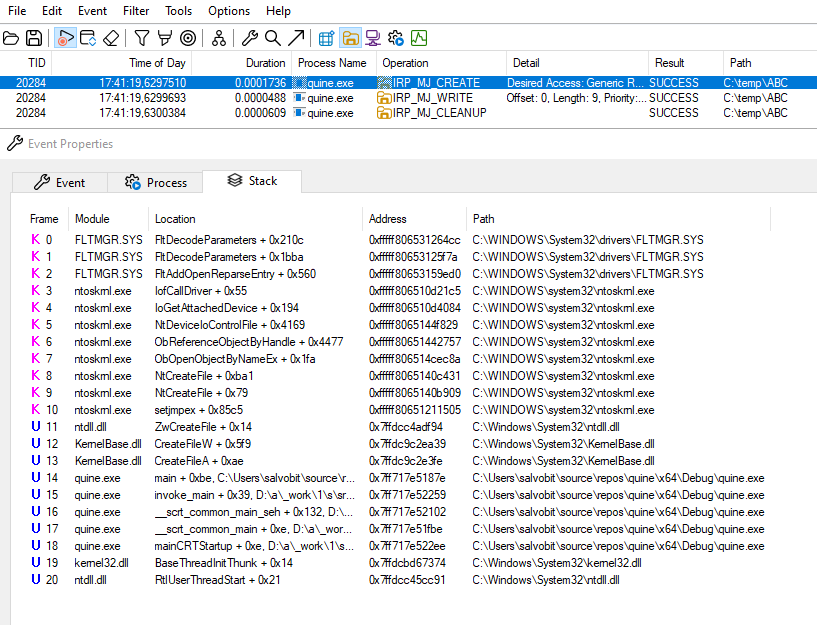
\includegraphics[height=0.72\textheight]{procmon-stack}
    \caption{Procmon (стек)}
  \end{figure}
\end{frame}

\section{Отговорности на ядрото}

\begin{frame}{Отговорности на ядрото}
  Ядрото стои между програмите и хардуера и отговаря за:
  \begin{itemize}
    \item управлението на процесите;
    \item управлението на паметта;
    \item управлението на входно-изходните устройства;
    \item управлението на устройствата за съхранение;
    \item защитата на системата.
  \end{itemize}
\end{frame}

\begin{frame}{Процеси}
  \begin{itemize}
    \item Процесът е програма по време на изпълнението ѝ. От една програма може
      да има много процеси едновременно - например два отворени терминала.
    \item Всеки процес има номер - PID, положително цяло число.
    \item Нов процес се създава с \texttt{fork()} - копие на родителя. Така
      процесите образуват дърво.
    \item С \texttt{execve()} процесът сменя програмата, която изпълнява.
    \item Първият процес, \texttt{init} (PID 1, днес обикновено
      \texttt{systemd}), се стартира от ядрото - всички останали произлизат от
      него.
  \end{itemize}
\end{frame}

\begin{frame}{Състояния на процес}
  \begin{center}
    \begin{tikzpicture}[
        font=\footnotesize,
        state/.style={draw=tuesnavy, fill=tuesblue!12, rounded corners=3pt,
          minimum width=2.3cm, minimum height=0.8cm},
        move/.style={->, >=stealth, thick, tuesnavy},
        why/.style={font=\scriptsize, text=black!75}]
      \node[state] (new) at (0,2.4) {Нов};
      \node[state] (ready) at (3.3,0.9) {Готов};
      \node[state] (running) at (8.4,0.9) {Изпълнява се};
      \node[state] (done) at (11.5,2.4) {Завършил};
      \node[state] (waiting) at (5.85,-1.6) {Чака};
      \draw[move] (new) -- node[why, sloped, above] {създаден} (ready);
      \draw[move] (ready.15) -- node[why, above] {избран от планировчика}
        (running.165);
      \draw[move] (running.195) -- node[why, below] {прекъсване от таймера}
        (ready.345);
      \draw[move] (running) |- node[why, pos=0.25, right] {чака вход-изход
        или събитие} (waiting);
      \draw[move] (waiting) -| node[why, pos=0.75, left] {събитието
        настъпи} (ready);
      \draw[move] (running) -- node[why, sloped, above] {\texttt{exit}}
        (done);
    \end{tikzpicture}
  \end{center}
\end{frame}

\begin{frame}{Смяна на състоянията}
  \begin{itemize}
    \item \emph{Готов $\to$ Изпълнява се} - планировчикът на ядрото му дава
      процесорно време.
    \item \emph{Изпълнява се $\to$ Готов} - времето му изтече. Ядрото запазва
      състоянието му (смяна на контекста, на англ. context switch), за да
      продължи по-късно оттам, където е спрял.
    \item \emph{Изпълнява се $\to$ Чака} - процесът сам чака нещо: вход от
      потребителя, данни от диска. Само изпълняващ се процес може да започне да
      чака.
    \item \emph{Чака $\to$ Готов} - събитието настъпи и процесът отново чака
      само процесор.
  \end{itemize}
\end{frame}

\begin{frame}{Край на процес}
  \begin{itemize}
    \item Процесът завършва сам (\texttt{exit}) или когато получи сигнал.
    \item \texttt{kill <pid>} изпраща сигнал - по подразбиране
      \texttt{SIGTERM}, който програмата може да прихване и да завърши
      спокойно. \texttt{SIGKILL} (\texttt{kill -9}) не може да бъде прихванат.
    \item Децата не завършват заедно с родителя си. Остават „сираци“ и
      получават нов родител - \texttt{init} (в Linux и процес, заявил, че
      осиновява сираци).
    \item ОС дава и механизми за комуникация (обмен на данни) и синхронизация
      между процесите - ще ги разгледаме по-нататък.
  \end{itemize}
\end{frame}

\begin{frame}{Управление на паметта}
  \begin{itemize}
    \item RAM е огромен масив от байтове с адреси. За да бъде изпълнена,
      програмата трябва да е в паметта.
    \item Ядрото:
      \begin{itemize}
        \item заделя и освобождава памет за процесите;
        \item следи коя част от паметта на кой процес принадлежи;
        \item решава кои данни да стоят в RAM и кои да се преместят на диска,
          когато паметта не стига.
      \end{itemize}
    \item Всеки процес вижда собствено (виртуално) адресно пространство -
      процесорът превежда адресите по таблици, поддържани от ядрото.
  \end{itemize}
\end{frame}

\begin{frame}{Управление на вход-изхода}
  \begin{itemize}
    \item Всяко устройство има драйвер, който знае как да работи с неговия
      контролер.
    \item Ядрото дава \emph{единен интерфейс} за цели видове устройства: в
      Unix устройствата са файлове в \texttt{/dev}, с които се работи с
      \texttt{read()} и \texttt{write()}. Програмата не се интересува от
      модела на устройството.
    \item Само ядрото има достъп до устройствата - инструкциите за вход-изход
      и адресите на контролерите са недостъпни в потребителски режим.
  \end{itemize}
\end{frame}

\begin{frame}{Буфериране, кеширане, спулинг}
  \begin{itemize}
    \item \emph{Буфер} - памет, в която данните чакат по пътя между
      устройството и програмата. Изглажда разликите в скоростта и в размера на
      порциите (дискът работи с блокове).
    \item \emph{Кеш} - копие на често използвани данни в по-бърза памет.
      Например ядрото държи прочетените части от файлове в RAM, за да не чете
      диска отново.
    \item \emph{Спулинг} - заданията към устройство, което обслужва само едно
      наведнъж, чакат в опашка. Когато няколко програми печатат едновременно,
      принтерът получава документите цели, един след друг.
  \end{itemize}
\end{frame}

\begin{frame}{Управление на съхранението}
  \begin{itemize}
    \item Устройствата за съхранение се различават по скорост, обем и начин на
      работа. Ядрото скрива разликите чрез две абстракции - \emph{файл} и
      \emph{файлова система}.
    \item Файлът е именувана поредица от байтове. Файловата система определя
      къде на устройството се намират те, а какво означават - решава
      програмата, която ги чете.
    \item Файловата система подрежда файловете в директории и пази правата за
      достъп. В Unix това са четене, писане и изпълнение - поотделно за
      собственика, групата и всички останали.
  \end{itemize}
\end{frame}

\begin{frame}{Защита}
  \begin{itemize}
    \item \textbf{Хардуерна}:
      \begin{itemize}
        \item режимите на процесора - привилегированите инструкции се
          изпълняват само в режим на ядрото;
        \item защита на паметта - всеки процес достъпва само своята памет (в
          най-простия вариант чрез регистрите BASE и LIMIT, днес - чрез
          таблиците на страниците);
        \item таймерът - ядрото си връща процесора, дори програма да зацикли.
      \end{itemize}
    \item \textbf{Софтуерна}: потребители и групи, права за достъп до
      файловете, проверка на всяко системно извикване.
  \end{itemize}
\end{frame}

\begin{frame}{Обобщение}
  \begin{itemize}
    \item Изложихме основните задачи, които решава една ОС.
    \item Уточнихме какво отличава ОС от библиотека за общо предназначение.
    \item Посочихме двата метода, чрез които ОС споделя ресурсите на машината.
    \item Разгледахме основната техника, използвана от ОС, за да изолират
      изпълнението на приложенията от хардуера.
    \item Видяхме как ОС постига многозадачност и многопотребителност.
    \item Разделихме ОС на ядро и потребителско пространство и изброихме
      отговорностите на ядрото.
  \end{itemize}
\end{frame}

\begin{frame}{За четене вкъщи}
  \footnotesize
  \begin{itemize}[<1->]
    \item \textcolor{tuesnavy}{Remzi H. Arpaci-Dusseau и Andrea C. Arpaci-Dusseau}.
      \emph{Introduction to Operating Systems}.
      {\color{bibnote}\url{https://pages.cs.wisc.edu/~remzi/OSTEP/intro.pdf}.
        Chapter from Operating Systems: Three Easy Pieces, Version 1.10. 2018}
    \item \textcolor{tuesnavy}{Remzi H. Arpaci-Dusseau и Andrea C. Arpaci-Dusseau}.
      \emph{Mechanism: Limited Direct Execution}.
      {\color{bibnote}\url{https://pages.cs.wisc.edu/~remzi/OSTEP/cpu-mechanisms.pdf}.
        Chapter from Operating Systems: Three Easy Pieces, Version 1.10. 2018}
    \item \textcolor{tuesnavy}{David Drysdale}. \emph{Anatomy of a system call, part 1}.
      {\color{bibnote}\url{https://lwn.net/Articles/604287/}. Article from
        LWN.net. 2014}
  \end{itemize}
\end{frame}

\begin{frame}
  \Large Край
\end{frame}

\end{document}
